\newpage
\chapter{METODE PENELITIAN} \label{Bab III}

\section{Alur Penelitian} \label{III.Alur}
Penelitian ini dilaksanakan melalui beberapa tahapan yang disusun secara berurutan agar proses pengolahan data dan eksperimen dapat berjalan dengan terstruktur. Setiap tahapan saling berkaitan satu sama lain, mulai dari pengumpulan dataset hingga analisis hasil klasifikasi. Gambaran umum mengenai alur penelitian yang dilakukan dapat dilihat pada Gambar \ref{fig:3.alur}. \par

\begin{figure}[H]
    \centering
    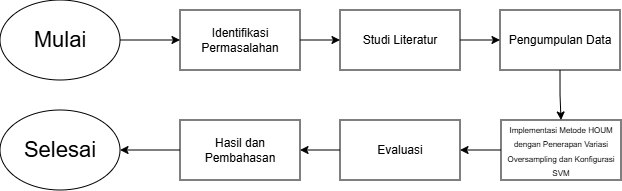
\includegraphics[width=1\textwidth]{figure/ALURPENELITIAN.png}
    \caption{Alur Penelitian}
    \label{fig:3.alur}
\end{figure}

\section{Penjabaran Langkah Penelitian} \label{III.Jabar Alur}
Bagian ini menjelaskan secara rinci setiap tahapan yang telah digambarkan pada Gambar \ref{fig:3.alur}. Penjelasan mencakup proses mulai dari identifikasi permasalahan, pengumpulan dataset, hingga tahapan akhir berupa analisis hasil eksperimen.

\subsection{Identifikasi Masalah} \label{III.Identifikasi_masalah}
Tahap awal penelitian dimulai dengan melakukan identifikasi terhadap permasalahan yang akan diteliti. Permasalahan utama yang melatarbelakangi penelitian ini adalah ketidakseimbangan distribusi kelas pada dataset klasifikasi, yang menyebabkan model \textit{machine learning} cenderung bias terhadap kelas mayoritas dan gagal mengenali kelas minoritas secara efektif \cite{He2009Imbalanced}. Eroglu dan Pir (2024) telah mengusulkan metode HOUM yang menggabungkan Safe-Level SMOTE dan SVM untuk menangani permasalahan ini, namun beberapa aspek dari metode tersebut belum dieksplorasi secara mendalam \cite{Eroglu2024HOUM}. Aspek pertama adalah pengaruh variasi parameter regularisasi $C$ dan jenis kernel pada komponen SVM terhadap kualitas proses \textit{undersampling}. Aspek kedua adalah perbandingan performa antara Safe-Level SMOTE yang digunakan pada HOUM asli dengan teknik \textit{oversampling} alternatif seperti ADASYN. Kedua aspek tersebut menjadi fokus utama yang akan dianalisis dalam penelitian ini untuk mengisi celah penelitian yang ada.

\subsection{Studi Literatur} \label{III.Studi_literatur}
Setelah permasalahan teridentifikasi, tahap selanjutnya adalah melakukan studi literatur untuk memahami konsep-konsep yang berkaitan dengan topik penelitian. Studi literatur dilakukan dengan mengkaji berbagai jurnal ilmiah, prosiding konferensi, dan artikel yang membahas tentang penanganan data tidak seimbang, teknik \textit{oversampling} dan \textit{undersampling}, serta metode hibrida. Beberapa topik utama yang dipelajari meliputi algoritma SMOTE beserta varian-variannya seperti Safe-Level SMOTE dan ADASYN, mekanisme kerja SVM sebagai algoritma klasifikasi dan perannya dalam proses \textit{undersampling}, serta metrik evaluasi yang sesuai untuk data tidak seimbang seperti ROC-AUC, G-mean, \textit{Recall}, dan \textit{Precision}. Kajian terhadap \textit{paper} HOUM oleh Eroglu dan Pir (2024) menjadi rujukan utama untuk memahami arsitektur metode dan mengidentifikasi celah penelitian yang belum dieksplorasi \cite{Eroglu2024HOUM}. Hasil dari studi literatur ini menjadi landasan dalam menyusun kerangka eksperimen dan menentukan variabel-variabel yang akan diuji pada penelitian ini.

\subsection{Pengumpulan Data} \label{III.Pengumpulan_data}
Dataset yang digunakan pada penelitian ini terdiri dari empat dataset \textit{benchmark}. Tiga dataset pertama, yaitu Diabetes, Haberman, dan Transfusion, merupakan dataset yang digunakan oleh Eroglu dan Pir (2024) dalam pengujian metode HOUM \cite{Eroglu2024HOUM}. Dataset keempat, yaitu Glass5, ditambahkan untuk menguji performa HOUM pada kondisi ketidakseimbangan yang tinggi. Keempat dataset tersebut dipilih karena memiliki karakteristik ketidakseimbangan kelas yang berbeda-beda, sehingga dapat merepresentasikan berbagai tingkat kesulitan dalam penanganan data tidak seimbang. Dataset diperoleh dari dua sumber publik yang umum digunakan dalam penelitian \textit{machine learning}, yaitu Kaggle dan UCI \textit{Machine Learning Repository}. Pemilihan tiga dataset yang sama dengan penelitian asli HOUM bertujuan agar hasil eksperimen dapat dibandingkan secara langsung dengan temuan sebelumnya, sedangkan penambahan Glass5 bertujuan untuk memperluas cakupan pengujian pada rasio ketidakseimbangan yang lebih tinggi. Ringkasan karakteristik keempat dataset ditunjukkan pada Tabel \ref{table:3.dataset}.

\begin{table}[H]
\centering
\caption{Karakteristik Dataset yang Digunakan}
\label{table:3.dataset}
\begin{tabular}{|l|c|c|c|c|c|}
\hline
\textbf{Dataset} & \textbf{Fitur} & \textbf{Instansi} & \textbf{Mayoritas} & \textbf{Minoritas} & \textbf{IR} \\
\hline
Diabetes & 9 & 768 & 500 & 268 & 1:1,87 \\
\hline
Haberman & 4 & 305 & 224 & 81 & 1:2,77 \\
\hline
Transfusion & 5 & 748 & 570 & 178 & 1:3,20 \\
\hline
Glass5 & 9 & 214 & 205 & 9 & 1:22,78 \\
\hline
\end{tabular}
\end{table}

Dataset Pima Indians Diabetes memuat data rekam medis pasien perempuan keturunan Pima Indian berusia minimal 21 tahun, dengan target klasifikasi berupa diagnosis positif atau negatif diabetes. Dataset ini memiliki 768 instansi dengan 9 fitur numerik yang mencakup informasi seperti jumlah kehamilan, konsentrasi glukosa plasma, tekanan darah, dan indeks massa tubuh. Rasio ketidakseimbangan pada dataset ini tergolong rendah yaitu 1:1,87 sehingga dapat merepresentasikan kondisi \textit{imbalance} tingkat rendah.

Dataset Haberman berisi data kelangsungan hidup pasien yang menjalani operasi kanker payudara di Rumah Sakit University of Chicago antara tahun 1958 hingga 1970. Dataset ini terdiri dari 305 instansi dengan 4 fitur yang meliputi usia pasien saat operasi, tahun operasi, dan jumlah kelenjar getah bening aksila positif yang terdeteksi. Target klasifikasi pada dataset ini adalah apakah pasien bertahan hidup selama lima tahun atau lebih setelah operasi. Rasio ketidakseimbangan sebesar 1:2,77 menempatkan dataset ini pada tingkat \textit{imbalance} yang sedikit lebih tinggi dibandingkan Diabetes.

Dataset Blood Transfusion Service Center memuat data donor darah yang dikumpulkan dari pusat layanan transfusi darah di Taiwan. Dataset ini terdiri dari 748 instansi dengan 5 fitur yang mencakup informasi seperti waktu sejak donasi terakhir (\textit{recency}), frekuensi donasi, total volume darah yang didonasikan, dan lama waktu sejak donasi pertama. Target klasifikasi berupa keputusan apakah donor akan mendonasikan darahnya pada periode berikutnya atau tidak. Rasio ketidakseimbangan sebesar 1:3,20 menempatkan dataset ini pada tingkat \textit{imbalance} yang lebih tinggi dibandingkan Diabetes dan Haberman.

Dataset Glass5 memuat data identifikasi jenis kaca berdasarkan komposisi kimianya. Dataset ini terdiri dari 214 instansi dengan 9 fitur numerik yang mencakup indeks bias (\textit{Refractive Index}), serta kandungan unsur kimia seperti Natrium (Na), Magnesium (Mg), Aluminium (Al), Silikon (Si), Kalium (K), Kalsium (Ca), Barium (Ba), dan Besi (Fe). Target klasifikasi pada dataset ini menentukan apakah suatu sampel kaca termasuk ke dalam kelas tertentu (kelas minoritas) atau bukan (kelas mayoritas). Rasio ketidakseimbangan sebesar 1:22,78 menjadikan dataset ini memiliki tingkat \textit{imbalance} yang paling tinggi diantara keempat dataset yang digunakan.

Masing-masing dataset dibagi menjadi dua bagian, yaitu data \textit{training} sebesar 80\% dan data uji sebesar 20\% menggunakan teknik \textit{stratified split} agar proporsi kelas pada kedua bagian tetap merepresentasikan distribusi kelas aslinya. Data uji disisihkan sejak awal dan tidak disentuh selama proses penyeimbangan berlangsung, sehingga evaluasi dilakukan pada data yang benar-benar belum pernah dilihat oleh model.

\subsection{Implementasi Metode HOUM dengan Variasi Oversampling dan Konfigurasi SVM} \label{III.Implementasi}
Tahap ini merupakan inti dari penelitian yang mencakup keseluruhan proses penerapan metode HOUM beserta variasi konfigurasi yang diuji. Alur implementasi secara lengkap digambarkan pada Gambar \ref{fig:3.flowimplementasi}. Proses dimulai dari pembagian data, dilanjutkan dengan penerapan \textit{undersampling} dan \textit{oversampling} secara iteratif, hingga akhirnya dilakukan klasifikasi dan perhitungan metrik performa.

\begin{figure}[H]
    \centering
    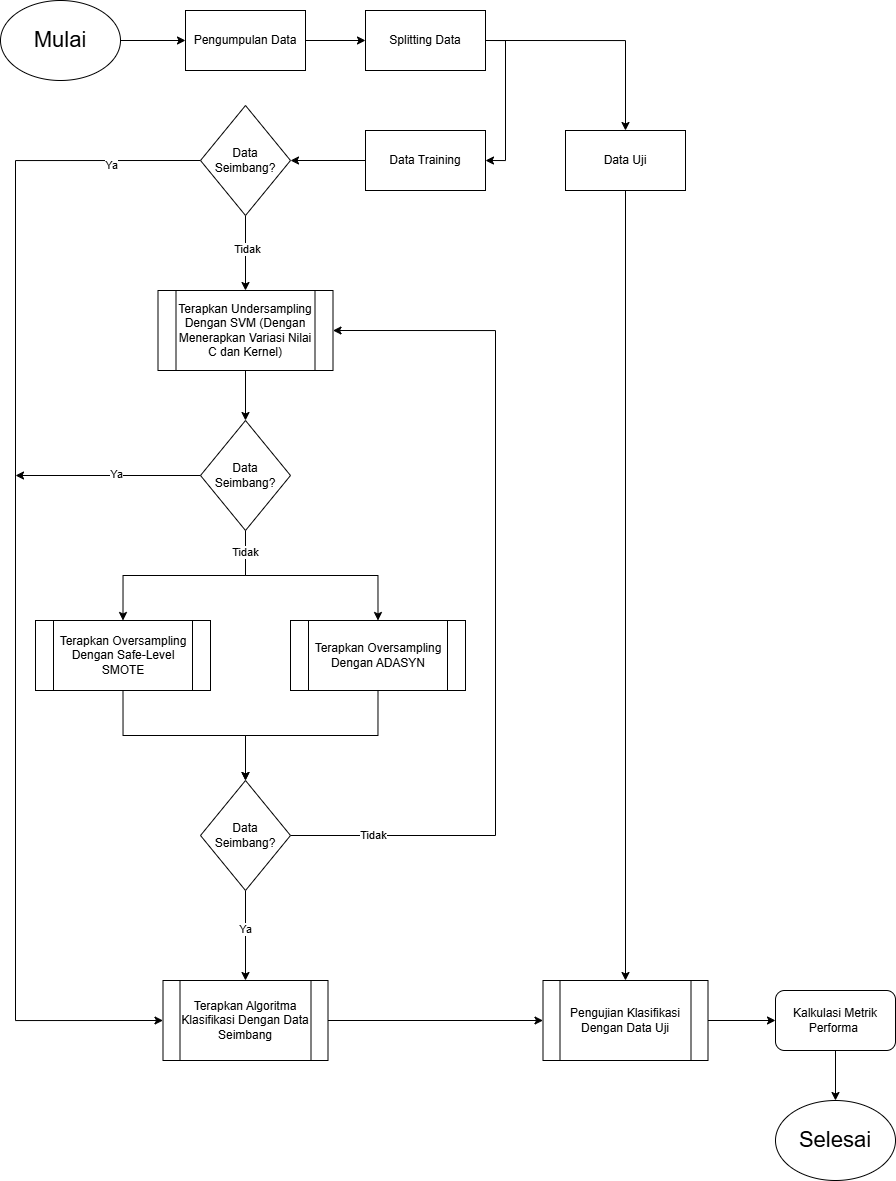
\includegraphics[width=0.9\textwidth]{figure/FlowImplementasi.png}
    \caption{Alur Implementasi Metode HOUM}
    \label{fig:3.flowimplementasi}
\end{figure}

Langkah pertama dalam implementasi adalah menggunakan data \textit{training} yang telah dipisahkan pada tahap pengumpulan data. Sebagai \textit{baseline}, data \textit{training} yang belum diseimbangkan (\textit{imbalanced}) langsung digunakan untuk melatih algoritma klasifikasi dan diuji pada data uji, sehingga diperoleh hasil performa tanpa penerapan metode HOUM sebagai pembanding.

Apabila data \textit{training} terdeteksi tidak seimbang, proses HOUM dimulai dengan tahap \textit{undersampling} menggunakan SVM. Pada tahap ini, SVM dilatih terlebih dahulu untuk membentuk \textit{decision boundary}, kemudian sampel kelas mayoritas yang berada jauh dari \textit{hyperplane} dihapus karena dianggap kurang informatif bagi proses klasifikasi. Setiap dataset diproses dengan seluruh kombinasi parameter SVM yang diuji, yaitu enam nilai parameter regularisasi $C$ (0,5; 1; 1,5; 2; 2,5; 3) dan tiga jenis kernel (Linear, RBF, Polynomial), sehingga menghasilkan 18 kombinasi konfigurasi \textit{undersampling} untuk setiap dataset.

Setelah tahap \textit{undersampling}, distribusi kelas diperiksa kembali. Apabila data masih belum seimbang, proses dilanjutkan ke tahap \textit{oversampling}. Pada tahap ini, masing-masing data hasil \textit{undersampling} dengan kombinasi kernel dan nilai $C$ tertentu diproses menggunakan dua teknik \textit{oversampling} secara terpisah, yaitu Safe-Level SMOTE sesuai metode HOUM asli dan ADASYN sebagai teknik alternatif. Dengan demikian, setiap kombinasi \textit{undersampling} menghasilkan dua varian data yang diseimbangkan melalui teknik \textit{oversampling} yang berbeda. Apabila setelah \textit{oversampling} data masih belum mencapai keseimbangan, proses diulang kembali ke tahap \textit{undersampling} secara iteratif hingga rasio antar kelas mencapai keseimbangan yang diharapkan.

Data yang sudah seimbang selanjutnya digunakan untuk melatih algoritma klasifikasi. Model yang telah dilatih kemudian diuji menggunakan data uji yang telah disisihkan pada tahap awal. Hasil pengujian dikalkulasi ke dalam metrik-metrik performa, yaitu ROC-AUC, G-mean, \textit{Recall}, dan \textit{Precision}. Contoh format keluaran hasil eksperimen untuk satu dataset ditunjukkan pada Tabel \ref{table:3.contohoutput}.

\begin{table}[H]
\centering
\caption{Contoh Format Keluaran Hasil Eksperimen}
\label{table:3.contohoutput}
\footnotesize
\begin{tabular}{|l|c|l|c|c|c|c|}
\hline
\textbf{Kernel} & \textbf{C} & \textbf{Tipe} & \textbf{ROC-AUC} & \textbf{Recall} & \textbf{Precision} & \textbf{G-Mean} \\
\hline
- & - & Imbalanced & 0,8118 & 0,5926 & 0,6809 & 0,7097 \\
\hline
linear & 0,50 & Balanced & 0,7956 & 0,6481 & 0,6140 & 0,7110 \\
\hline
linear & 1,00 & Balanced & 0,8264 & 0,6111 & 0,6226 & 0,6992 \\
\hline
linear & 1,50 & Balanced & 0,8081 & 0,6296 & 0,6182 & 0,7053 \\
\hline
linear & 2,00 & Balanced & 0,8035 & 0,6852 & 0,6271 & 0,7311 \\
\hline
linear & 2,50 & Balanced & 0,7969 & 0,6296 & 0,6296 & 0,7097 \\
\hline
linear & 3,00 & Balanced & 0,7912 & 0,6481 & 0,6087 & 0,7054 \\
\hline
\end{tabular}
\end{table}

Pada tabel tersebut, baris dengan tipe \textit{Imbalanced} menunjukkan hasil \textit{baseline} di mana data langsung diklasifikasikan tanpa melalui proses penyeimbangan HOUM. Baris ini hanya ditampilkan satu kali karena tidak melibatkan variasi parameter apapun. Baris dengan tipe \textit{Balanced} menunjukkan hasil setelah data diseimbangkan menggunakan metode HOUM dengan kombinasi kernel dan nilai $C$ yang bersangkutan. Perbandingan antara baris \textit{Imbalanced} dan \textit{Balanced} menunjukkan dampak penerapan HOUM terhadap performa klasifikasi pada masing-masing konfigurasi.

\subsection{Evaluasi} \label{III.Evaluasi}
Tahap evaluasi bertujuan untuk menganalisis dan membandingkan hasil metrik performa dari seluruh skenario eksperimen yang telah dijalankan. Perbandingan dilakukan dari beberapa sudut pandang, yaitu pengaruh variasi nilai parameter $C$ terhadap performa klasifikasi pada masing-masing jenis kernel, pengaruh pemilihan jenis kernel pada setiap nilai $C$, serta perbandingan performa antara HOUM yang menggunakan Safe-Level SMOTE dengan HOUM yang menggunakan ADASYN. Selain itu, perbandingan antara hasil \textit{baseline} (\textit{imbalanced}) dan hasil setelah penyeimbangan (\textit{balanced}) dilakukan untuk mengukur seberapa besar kontribusi metode HOUM dalam meningkatkan kemampuan klasifikasi kelas minoritas. Evaluasi dilakukan secara konsisten pada keempat dataset untuk melihat apakah tren yang ditemukan bersifat umum atau spesifik terhadap karakteristik dataset tertentu.

\subsection{Hasil dan Pembahasan} \label{III.HasilPembahasan}
Tahap terakhir dari alur penelitian ini adalah penyajian hasil eksperimen beserta pembahasannya. Hasil performa dari seluruh kombinasi konfigurasi ditampilkan dalam bentuk tabel dan grafik perbandingan agar pola yang terbentuk dapat diamati dengan jelas. Pembahasan mencakup interpretasi terhadap temuan eksperimen, identifikasi konfigurasi HOUM yang menghasilkan performa terbaik, serta analisis mengenai mengapa konfigurasi tertentu menghasilkan performa yang lebih baik atau lebih buruk pada dataset tertentu. Temuan dari penelitian ini kemudian dibandingkan dengan hasil yang dilaporkan oleh Eroglu dan Pir (2024) untuk menilai konsistensi dan kontribusi dari variasi konfigurasi yang diuji \cite{Eroglu2024HOUM}. Kesimpulan dan rekomendasi konfigurasi optimal disusun berdasarkan analisis menyeluruh terhadap seluruh hasil eksperimen.

\section{Alat dan Bahan Tugas Akhir} \label{III.Alat dan Bahan}
Perangkat lunak yang digunakan dalam penelitian ini adalah Jupyter Notebook dengan bahasa pemrograman Python untuk implementasi metode, menjalankan eksperimen, dan melakukan pengujian terhadap hasil klasifikasi. Sedangkan bahan yang digunakan dalam penelitian ini terdiri dari empat dataset, yaitu Pima Indians Diabetes, Haberman, Blood Transfusion Service Center, dan Glass5 yang diperoleh dari situs Kaggle dan UCI \textit{Machine Learning Repository}, serta referensi jurnal dan artikel ilmiah terdahulu yang berkaitan dengan topik penelitian.

\section{Rancangan Pengujian} \label{III.Pengujian}

Pengujian pada penelitian ini dilakukan dengan menggunakan algoritma \textit{Random Forest} sebagai metode klasifikasi dari pustaka \textit{Scikit-Learn} dengan seluruh parameter \textit{default} yang sudah disediakan oleh \textit{Scikit-Learn}. Penggunaan parameter default dilakukan untuk menjaga fokus penelitian pada analisis pengaruh variasi konfigurasi metode HOUM, sehingga perubahan performa yang diperoleh lebih menunjukkan dampak proses penyeimbangan data dibandingkan proses optimasi model klasifikasi. Algoritma \textit{Random Forest} dipilih karena merupakan algoritma \textit{ensemble learning} yang menggabungkan beberapa \textit{decision tree} untuk menghasilkan prediksi yang lebih stabil dan akurat dibandingkan penggunaan satu \textit{decision tree} tunggal. Algoritma ini memiliki ketahanan yang baik terhadap \textit{overfitting} dan mampu menangani data dengan jumlah fitur yang beragam. 

Model \textit{Random Forest} dilatih menggunakan data \textit{training} yang telah melalui proses penyeimbangan HOUM, kemudian diuji pada data uji yang telah disisihkan sejak awal. Sebagai pembanding, model juga dilatih menggunakan data \textit{training} asli yang belum diseimbangkan (\textit{imbalanced}) untuk mengukur kontribusi metode HOUM terhadap peningkatan performa klasifikasi. Hasil prediksi dari model klasifikasi kemudian dievaluasi menggunakan beberapa metrik evaluasi, yaitu \textit{Recall}, \textit{Precision}, G-Mean, dan ROC-AUC. Metrik-metrik ini dipilih karena mampu memberikan gambaran kinerja model secara lebih menyeluruh, terutama pada kasus data tidak seimbang.
